%%%%%%%%%%%%%%%%%%%%%%%%%%%%%%%%%%%%%%%%%%%%%%%%%%%%%%%%%%%%%%%%%%%%%%%%
% TFG: Vigilancia Tecnológica y Minería de Opiniones en RRSS
% Escuela Técnica Superior de Ingenierías Informática y de Telecomunicación
% Realizado por: Miguel Keane Cañizares
% Contacto: miguekeca@correo.ugr.es 
%%%%%%%%%%%%%%%%%%%%%%%%%%%%%%%%%%%%%%%%%%%%%%%%%%%%%%%%%%%%%%%%%%%%%%%%

\chapter{Resultados}

De los varios scripts implementados, se han obtenido una gran gama de resultados. Las pruebas han sido orientadas hacia servicios de Streaming Online, debido a que son empresas que están a la orden del día y generan gran actividad en las redes sociales. Con el deseo de buscar una finalidad práctica para realizar un estudio de mercado. Se ha utilizado un formato de \"carreras\" donde se han seleccionado dos plataformas, para las cuales se han ejecutado dos procesos paralelos, cada uno creando una base de datos sobre una plataforma concreta. De esta forma a parte de los resultados de la polaridad, también se puede medir el tráfico de datos que genera su red social con respecto a su competencia. La API de Twitter nos permite hacer dos escuchas simultáneas, por lo que no es necesario hacer uso de más cuentas. 

En total fueron bastantes las bases de datos generadas con las diferentes pruebas, las bases de datos MongoDB generadas fueron las siguientes:


\begin{figure}[H]
	\centering
	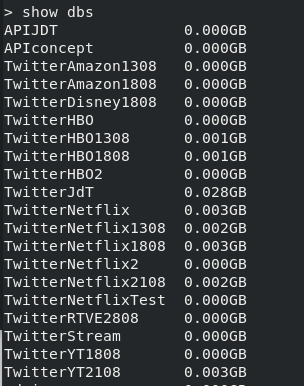
\includegraphics[scale=.5]{imagenes/BD-Mongo.png}
	\caption{Diferentes BD generadas en MongoDB}
	\label{fig:BD-MongoDB}
\end{figure}


\section{Análisis de Netflix y HBO}
Al ser las dos plataformas principales y grandes competidoras entre sí, han sido el objeto principal de las pruebas del proyecto.

La primera competencia fue el día 13 de Agosto, de 22h a 1h. Tres horas donde fueron descargados por separados aquellos tweets que mencionaban Netflix y los que mencionaban a HBO, guardados en diferentes bases de datos. 

\begin{figure}[H]
	\centering
	\begin{tabular}{c c}
		
		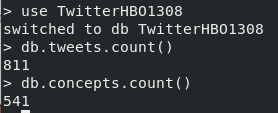
\includegraphics[scale=.62]{imagenes/HBO1308Mongo.png}
		&  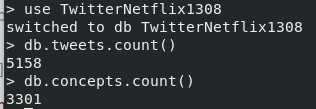
\includegraphics[scale=.65]{imagenes/Netflix1308Mongo.png} \\ 
		
		{BD de HBO1308}
		
		&  {BD de Netflix1308} \\ 
		
	\end{tabular} 
	\label{fig:Mongo1308}
\end{figure}

Aquí podemos apreciar dos colecciones en cada base de datos. La primera \textit{tweets} son el total de tweets capturados por el \textit{ladrón de tweets}, la otra \textit{concepts} son el resultados del análisis de haberlo enviado a MeaningCloud con el \textit{analisis-sentimientos-mongo}. Lo principal que se puede apreciar es que Netflix tiene mucha más presencia en redes que HBO, puesto que es mencionado más de 5 veces por cada vez que se menciona a HBO. 

Tambiés es notable como el número de tweets que han sido analizados es mucho más bajo que los capturados. Esto es debido principalmente a que MeaningCloud no admite emojis en su análisis y siendo estos tan presentes en las redes hay una notable pérdida de información a la hora de analizarla. En este caso los tweets de HBO han tenido una tasa del 66,7\% de tweets analizables mientras que Netflix tiene una tasa del 64\%. La diferencia es casi despreciable. 


Pasando a estudiar los resultados del análisis de sentimientos, obtenemos lo siguiente. 

\begin{table}[H]
	\centering
	\begin{tabular}{|c|c|c|}
		\hline 
		Polaridad& Suma de polaridades & Porcentaje \\ 
		\hline 
		N+& 36 & 10,62\% \\ 
		\hline 
		N& 90 &  26,55\%\\ 
		\hline 
		NEU& 17 & 5,01\% \\ 
		\hline 
		P& 154 & 45,43\% \\ 
		\hline 
		P+& 42 & 12,39\% \\ 
		\hline 
		Total & 339 & \\
		\hline
	\end{tabular} 
	\caption{Tabla de porcentajes de HBO1308}
	\label{tbl:porcentaje-HBO1308}
\end{table}



La razón por la que en el total de aparece la cifra de 339 en vez de 541 es porque 202 tweets han sido clasificados como NONE, es decir, sin ninguna polaridad emocional detectada. Esto correspondería al 37\% de los tweets analizados.

\begin{table}[H]
	\centering
	\begin{tabular}{|c|c|c|}
		\hline 
		Polaridad& Suma de polaridades & Porcentaje \\ 
		\hline 
		N+& 292 & 14,37\% \\ 
		\hline 
		N& 920 &  42,28\%\\ 
		\hline 
		NEU& 134 & 6,59\% \\ 
		\hline 
		P& 527 & 25,94\% \\ 
		\hline 
		P+& 159 & 7,82\% \\ 
		\hline 
		Total & 2032 & \\
		\hline
		
	\end{tabular} 
	\caption{Tabla de porcentajes de Netflix1308}
	\label{tbl:porcentaje-Netflix1308}
\end{table}
\begin{figure}[H]
	
\end{figure}



En Netflix el 38\% de los tweets analizados no tenían polaridad. Equivalente a 1269 tweets de los 3301 estudiados. 

A continuación ilustraremos unos gráficos de los resultados: 

\begin{figure}[H]
	\centering
	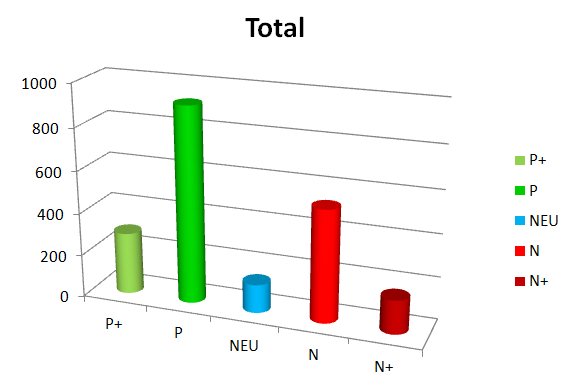
\includegraphics[scale=.3]{imagenes/GraficoBarrasNetflix1308.PNG}
	\caption{Gráfico de barras de Netflix1308}
	\label{fig:barrasNetflix1308}
\end{figure}


\begin{figure}[H]
	\centering
	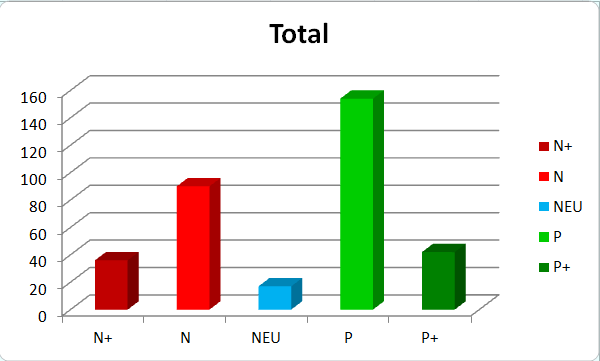
\includegraphics[scale=.3]{imagenes/barrasHBO1308.PNG}
	\caption{Gráfico de barras de HBO1308}
	\label{fig:barrasHBO1308}
\end{figure}

Con estos resultados podemos apreciar que la mayoría de los tonos emocionales detectados son Negativos o Positivos, siendo los positivos la mayoría tanto en Netflix como en HBO. 


El siguiente análisis fue realizado el 18 de Agosto de 2019. desde las 0:20 hasta las 3am. Un total de dos horas y cuarenta minutos. 

\begin{figure}[H]
	\centering
	\begin{tabular}{c c}
		
		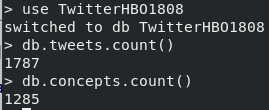
\includegraphics[scale=.7]{imagenes/HBO1808Mongo.png}
		&  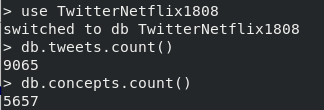
\includegraphics[scale=.7]{imagenes/Netflix1808Mongo.png} \\ 
		
		{BD de HBO1808}
		
		&  {BD de Netflix1808} \\ 
		
	\end{tabular} 
	\label{fig:Mongo1808}
\end{figure}

Netflix no deja lugar a dudas, vuelve a tener 5 veces más tráfico en las redes que su rival HBO. 
En esta ocasión, HBO ha tenido un 72\% de tweets sin emojis y Netflix se mantiene casi igual que antes con un 62\%. Analizando los resultados uno por uno se observa lo siguiente: 

\begin{table}[H]
	\centering
	\begin{tabular}{|c|c|c|}
		\hline 
		Polaridad& Suma de polaridades & Porcentaje \\ 
		\hline 
		N+& 265 & 7.87\% \\ 
		\hline 
		N& 815 &  24.21\%\\ 
		\hline 
		NEU& 237 & 7.04\% \\ 
		\hline 
		P& 1435 & 42.63\% \\ 
		\hline 
		P+& 614 & 18.24\% \\ 
		\hline 
		Total & 3366 & \\
		\hline
	\end{tabular} 
	\caption{Tabla de porcentajes de Netflix1808}
	\label{tbl:porcentaje-Netflix1808}
\end{table}

En Netflix a 2291 tweets, es decir, al 60\% de los analizados, no se le ha detectado tono emocional alguno. 

\begin{table}[H]
	\centering
	\begin{tabular}{|c|c|c|}
		\hline 
		Polaridad& Suma de polaridades & Porcentaje \\ 
		\hline 
		N+& 73 & 9.22\% \\ 
		\hline 
		N& 220 &  27.78\%\\ 
		\hline 
		NEU& 67 & 8.46\% \\ 
		\hline 
		P& 357 &45.08\% \\ 
		\hline 
		P+& 75 & 9.47\% \\ 
		\hline 
		Total & 792 & \\
		\hline
	\end{tabular} 
	\caption{Tabla de porcentajes de HBO1808}
	\label{tbl:porcentaje-HBO1808}
\end{table}
HBO ha tenido 493 tweets sin tono emocional, equivalente aproximadamente al 38\% del total analizado. 


Las gráficas obtenidas son las siguientes: 

\begin{figure}[H]
	\centering
	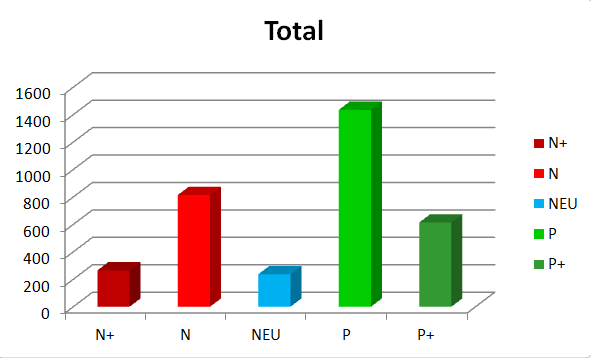
\includegraphics[scale=.3]{imagenes/barrasNetflix1808.PNG}
	\caption{Gráfico de barras de Netflix1808}
	\label{fig:barrasNetflix1808}
\end{figure}



\begin{figure}[H]
	\centering
	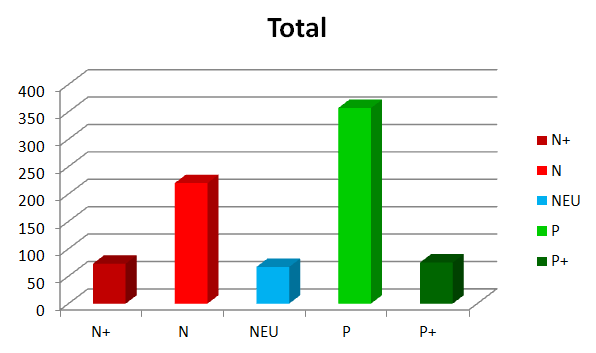
\includegraphics[scale=.3]{imagenes/barrasHBO1808.PNG}
	\caption{Gráfico de barras de HBO1808}
	\label{fig:barrasHBO1808}
\end{figure}


Aquí se observa la misma tendencia anterior, la inmensa mayoría de la polaridad emocional es para expresar un tono positivo o negativo, pocos expresan polaridades extremas o neutras. Con la diferencia de que en HBO hay un incremento del porcentaje de opiniones negativas con respecto a Netflix y Netflix porcentualmente recibe cerca del doble de tonos muy positivos. 


\subsection{Netflix vs Youtube}

Al haber observado que Netflix poseía una abrumadora superioridad en cuanto a número de usuarios y actividad en las redes que HBO, se optó por hacerla competir con una plataforma mucho más grande, como puede ser YouTube. YouTube es otro formato de plataforma de Streaming Online, pero a diferencia de Netflix y HBO su contenido es gratuito y creado por los propios usuarios, aunque recientemente se ha presentado al público YouTube Premium, cuya ventaja es la de suprimir los anuncios, han aprovechado para empezar a ofrecer contenido cinematográfico exclusivo para sus suscriptores, es decir, series y películas producidas por la compañía de Google, como llevan muchos años haciendo Netflix y HBO. 

Se les analizó el 21 de Agosto de 2019, de las 16h hasta las 17:30h. Una hora y media de escucha.


 
 \begin{figure}[H]
 	\centering
 	\begin{tabular}{c c}
 		
 		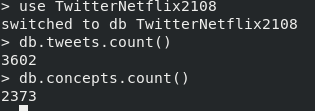
\includegraphics[scale=.7]{imagenes/Netflix2108Mongo.png}
 		&  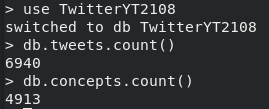
\includegraphics[scale=.7]{imagenes/YT2108Mongo.png} \\ 
 		
 		{BD de Netflix2108}
 		
 		&  {BD de YouTube2108} \\ 
 		
 	\end{tabular} 
 	\label{fig:Mongo2108}
 \end{figure}


Es apreciable, que siempre hay un pez más grande. YouTube en tan solo hora y media es mencionada el doble de veces que Netflix.  Netflix mantiene su línea de contenido sin emojis, un 65,8\% de todos los tweets son analizables, mientras que YouTube se mantiene superior, con un 70\% de éxito en los tweets que se analizan correctamente. 



\begin{table}[H]
	\centering
	\begin{tabular}{|c|c|c|}
		\hline 
		Polaridad& Suma de polaridades & Porcentaje \\ 
		\hline 
		N+& 96 & 6.71\% \\ 
		\hline 
		N& 358 &  25.02\%\\ 
		\hline 
		NEU& 102 & 7.13\% \\ 
		\hline 
		P& 646 & 45,14\% \\ 
		\hline 
		P+& 229 & 16.00\% \\ 
		\hline 
		Total & 1431 & \\
		\hline
	\end{tabular} 
	\caption{Tabla de porcentajes de Netflix2108}
	\label{tbl:porcentaje-Netflix2108}
\end{table}

En Netflix ha habido 942 tweets sin tono emocional, lo que equivale al 39,69\% de los analizados. 

\begin{table}[H]
	\centering
	\begin{tabular}{|c|c|c|}
		\hline 
		Polaridad& Suma de polaridades & Porcentaje \\ 
		\hline 
		N+& 238 & 8.38\% \\ 
		\hline 
		N& 773 &  27.22\%\\ 
		\hline 
		NEU& 135 & 4.75\% \\ 
		\hline 
		P& 1327 & 46.73\% \\ 
		\hline 
		P+& 367 & 12.92\% \\ 
		\hline 
		Total & 2840 & \\
		\hline
	\end{tabular} 
	\caption{Tabla de porcentajes de YouTube2108}
	\label{tbl:porcentaje-YT2108}
\end{table}

En YouTube hubo 2073 tweets carentes de tono emocional, 42,12\% del total. 


\begin{figure}[H]
	\centering
	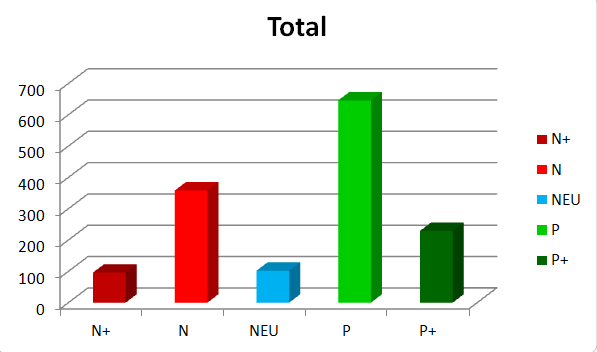
\includegraphics[scale=.3]{imagenes/barrasNetflix2108.PNG}
	\caption{Gráfico de barras de Netflix2108}
	\label{fig:barrasNetflix2108}
\end{figure}



\begin{figure}[H]
	\centering
	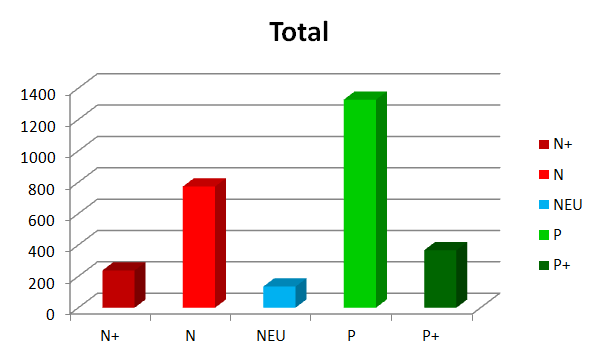
\includegraphics[scale=.3]{imagenes/barrasYT2108.PNG}
	\caption{Gráfico de barras de YouTube2108}
	\label{fig:barrasYT2108}
\end{figure}


En cuanto a las gráficas se refieren, no hay diferencias notables entre las dos plataformas. Se mantiene el tono positivo a la cabeza con el negativo detrás. Aunque levemente, en YouTube hay un mayor porcentaje de tonos extremos, es decir, hay más tonos muy positivos y tonos muy negativos que en Netflix. 



\subsection{Estudio del total analizado}
Uniendo todos los tweets analizados en ficheros únicos gracias al script \textit{unificador-csv} para poder analizar los resultados completos.


\textbf{Netflix: }

\begin{table}[H]
	\centering
	\begin{tabular}{|c|c|c|}
		\hline 
		Polaridad& Suma de polaridades & Porcentaje \\ 
		\hline 
		N+& 520 & 7.61\% \\ 
		\hline 
		N& 1700 &  24.89\%\\ 
		\hline 
		NEU& 473 & 6.93\% \\ 
		\hline 
		P& 3001 & 43.94\% \\ 
		\hline 
		P+& 1135 & 16.62\% \\ 
		\hline 
		Total & 6829 & \\
		\hline
	\end{tabular} 
	\caption{Tabla de porcentajes de Netflix total}
	\label{tbl:porcentaje-NetflixAll}
\end{table}

 \begin{figure}[H]
	\centering
	
	 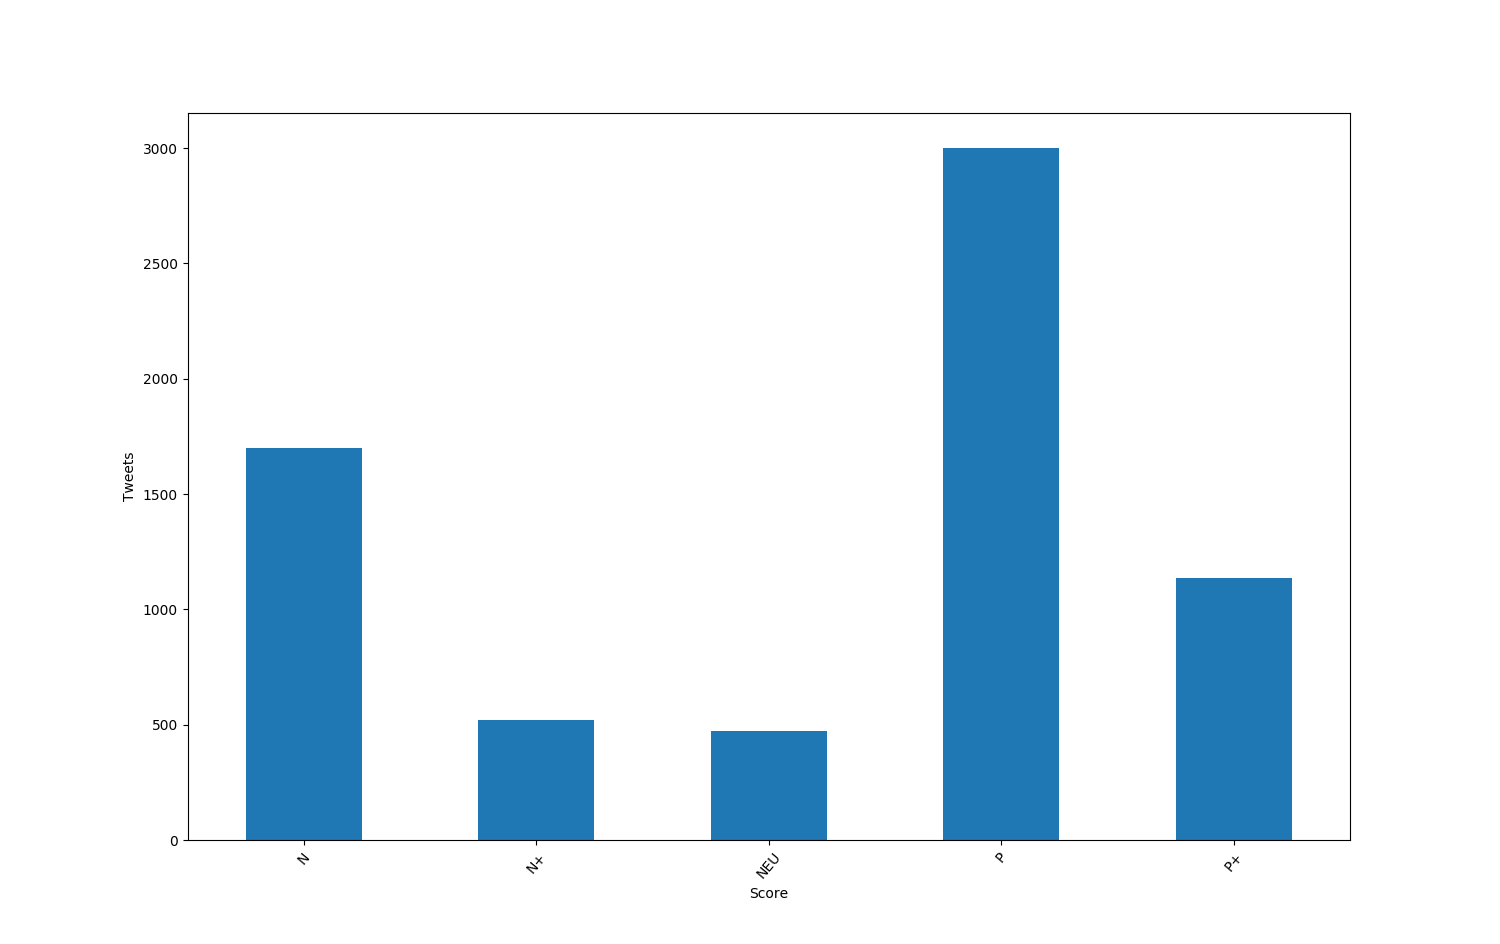
\includegraphics[scale=.3]{imagenes/barrasNetflixAll.png}
		
	
		
	\caption{Gráfico de barras de Netflix total} 
	\label{fig:NetflixAll}
\end{figure}





Es claramente apreciable que la gran mayoría de los comentarios de Netflix son positivos y muy positivos. Hay más comentarios negativos que muy positivos,  pero la diferencia es mínima y siendo solo el 39\% del total positivo es superior al 19\% que suman los tweets negativos y muy negativos. 




\textbf{HBO: }


\begin{table}[H]
	\centering
	\begin{tabular}{|c|c|c|}
		\hline 
		Polaridad& Suma de polaridades & Porcentaje \\ 
		\hline 
		N+& 116 & 26.76\% \\ 
		\hline 
		N& 320 &  9.70\%\\ 
		\hline 
		NEU& 90 & 7.53\% \\ 
		\hline 
		P& 547 & 45.74\% \\ 
		\hline 
		P+& 123 & 10.28\% \\ 
		\hline 
		Total & 1196 & \\
		\hline
	\end{tabular} 
	\caption{Tabla de porcentajes de HBO total}
	\label{tbl:porcentaje-HBOAll}
\end{table}

\begin{figure}[H]
	\centering
		
		 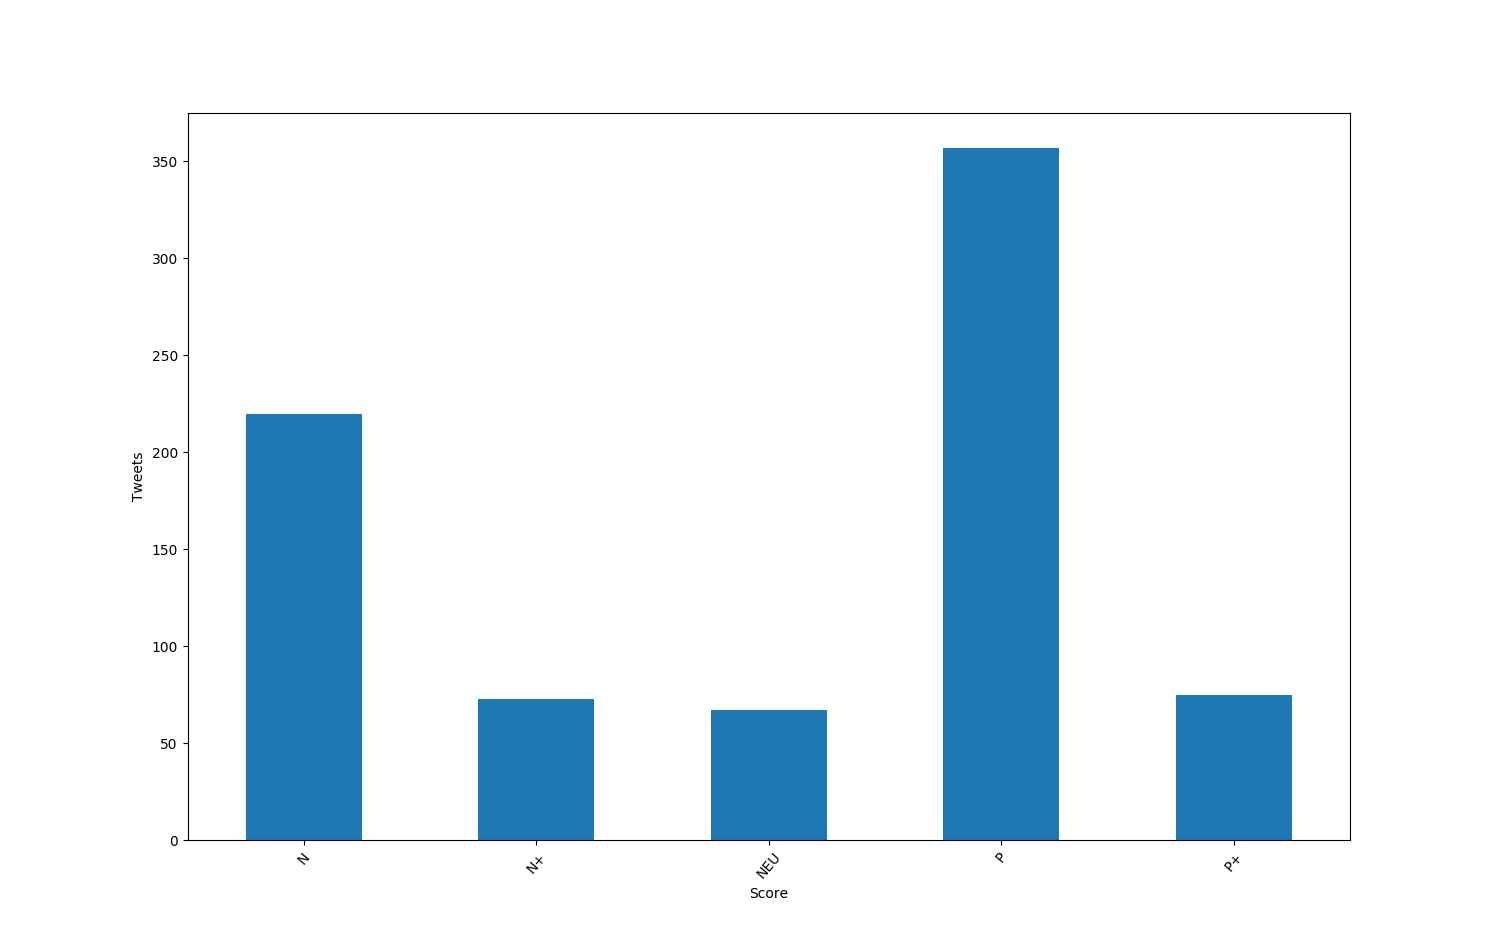
\includegraphics[scale=.3]{imagenes/barrasHBOAll.png} 
		
		{Porcentajes de HBO total}
		
	\caption{Gráfico de barras de HBO total} 
		
	\label{fig:HBOAll}
\end{figure}



La tendencia es similar a la de Netflix, puesto que la mayoría de comentarios son positivos y se evitan los extremos y los neutros. Pero en HBO la diferencia entre positivos y negativos es menor, es decir, hay una mayor porcentaje de usuarios que escriben comentarios negativos al hablar de HBO. 



\subsection{Disney+ y AmazonVideos}

También, como dato anecdótico, se intentó hacer competir la repercusión en redes de la plataforma que va a sacar Disney al mercado, Disney+, y la plataforma de Amazon, AmazonVideos. Pero los resultados fueron poco alentadores, con apenas 150 tweets de Disney+ publicados durante la captación y tan solo 3 tweets de AmazonVideos en el mismo espacio, cabe notar que los tweets de Amazon fueron todos publicados por un mismo usuario repitiendo un mismo mensaje. 



\subsection{WordClouds}
Las nubes de palabras son una forma útil para analizar los datos obtenidos. Con esta forma podemos crear un resumen visual de los datos obtenidos, obteniendo las palabras más utilizadas en la base de datos almacenada. 


Inicialmente las nubes de palabras se veían así: 

\begin{figure}[H]
	\centering
	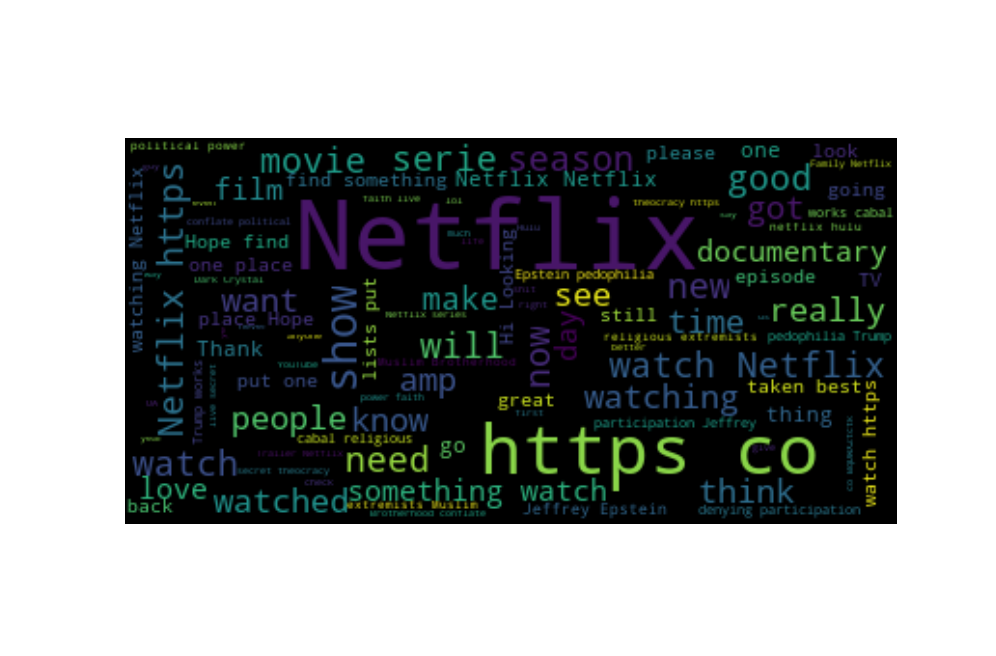
\includegraphics[scale=.5]{imagenes/WordCloudNetflix1.png}
	\caption{Primer WordCloud de Netflix}
	\label{fig:wordcloudNetflix1}
\end{figure} 

El primer fallo notable era que la palabra \textit{Netflix} aparecía muy repetida, lo cual es obvio, pues esta era la palabra clave utilizada para descargar los tweets, es decir, todos ellos la contenían. Además, un gran número de tweets incluye enlaces, al empezar todos los enlaces por https el algoritmo detectó esta palabra apareciendo repetidas veces. Además se detectó \textit{amp}, utilizado por caracteres especiales y \textit{co} que figura en los enlaces. Implementando el uso de stopwords y cambiando el fondo a blanco por limpieza visual el resultado fue el siguiente: 

\begin{figure}[H]
	\centering
	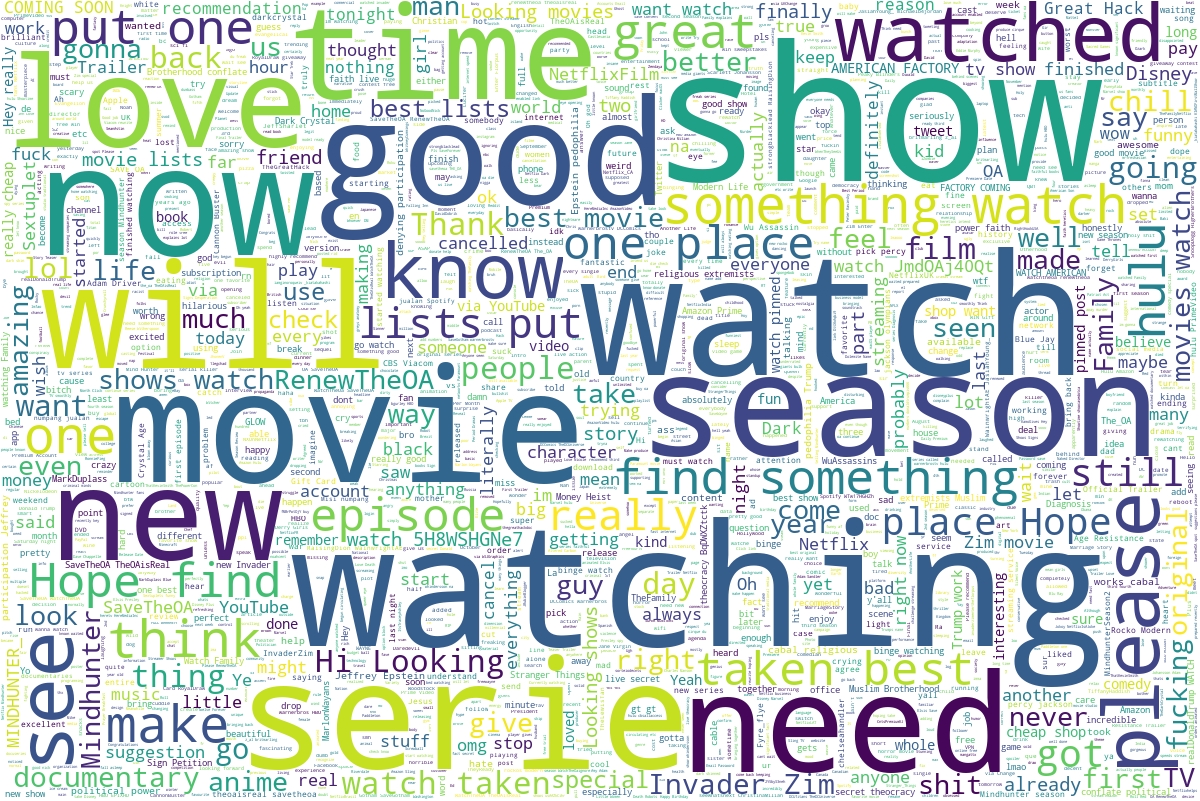
\includegraphics[scale=.3]{imagenes/NetflixAll.png}
	\caption{Segundo WordCloud de Netflix}
	\label{fig:wordcloudNetflix2}
\end{figure} 

En esta segunda versión, se aumenta el número de palabras representadas y el uso de StopWords para limpiar los resultados. Los resultados obtenidos son los que nos podíamos esperar del análisis de un wordcloud de Netflix, palabras como watch, movie, season entre otras están presentes. Es notable como leyendo los resultados se puede extrapolar como la mayoría de usuarios lo utiliza para hablar de series y programas que le gustan: love, good, watch, now. Y como también hay otros usuarios que comentan para recibir recomendaciones: something watch ,  please, Looking. 

Lo mismo sucedía con los demás, por lo que adaptando las palabras claves este era el resultado: 

\begin{figure}[H]
	\centering
	\includegraphics[scale=.8]{imagenes/ytwords.png}
	\caption{Primer WordCloud de YouTube}
	\label{fig:wordcloudYT1}
\end{figure} 

Y excluyendo la palabra YouTube: 

\begin{figure}[H]
	\centering
	\includegraphics[scale=.8]{imagenes/ytstopwords.png}
	\caption{Segundo WordCloud de YouTube}
	\label{fig:wordcloudYT2}
\end{figure} 


Aquí es apreciable una diferencia del formato. Ya no se ven palabras como season, movie o serie. Las cuales se ven reemplazadas por video, song, subscribe o play. Google, dueña de YouTube aparece mencionada en muchas ocasiones. 
 
Para el estudio de la nube de HBO, además de cambiar los colores se cambiaron los contornos, para mostrar las posibilidades estéticas que permite el manejo de la librería \textbf{PIL}\cite{Pillow}. Siendo posible la creación de nubes con diferentes formas. 

\begin{figure}[h]
	\centering
	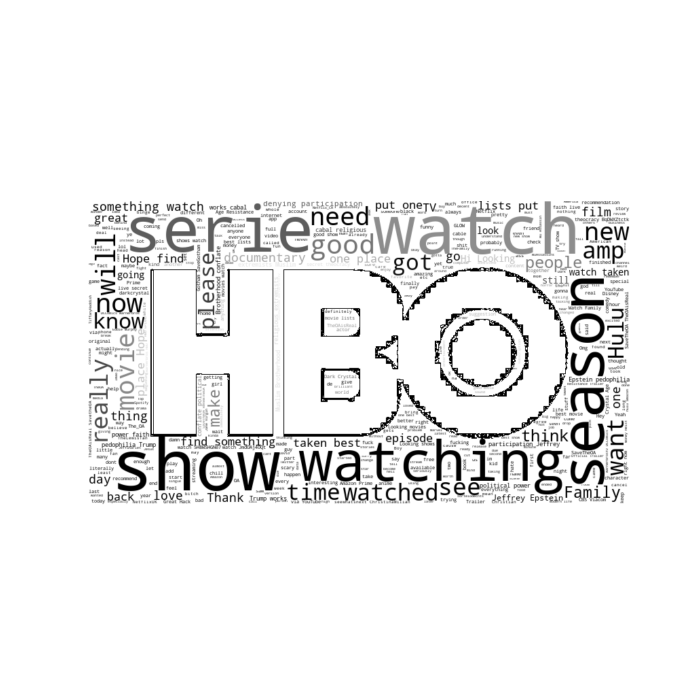
\includegraphics[scale=.75]{imagenes/hbo_color2.png}
	\caption{WordCloud de HBO}
	\label{fig:wordcloudHBO}
\end{figure} 

En cuanto a las palabras, no se aprecia gran diferencia con respecto a las de Netflix, al ser un servicio parecido, inevitablemente aparecen palabras similares. Con el detalle de que aparece mencionada la plataforma Hulu, la cual tras una breve búsqueda en Google podemos averiguar que en Estados Unidos esta plataforma ofrece los servicios de HBO de la misma forma que Movistar ofrece Netflix en España. 




\subsection{Juego de Tronos}

Como añadido, durante la semana del final del último capítulo de la serie Juego de Tronos hubo una versión previa del \textit{ladrón de tweets}, capturó más de 170mil tweets solo en dos días, el problema es que no esta versión no disponía de un filtro para evitar los Retweets, por lo que la inmensa mayoría de la información es el mismo tweet repetido una y otra vez. Además no estaba gestionado el modo extendido para capturar tweets de más de 140 caracteres. Por lo que su utilidad real para el análisis de sentimientos es escasa, pero aún así se ha realizado un wordcloud y un análisis de sentimientos parcial, pues el número de tweets era abrumador. 



El total de palabras analizadas es de 19.809.698, las cuales generan el siguiente wordcloud:

\begin{figure}[H]
	\centering
	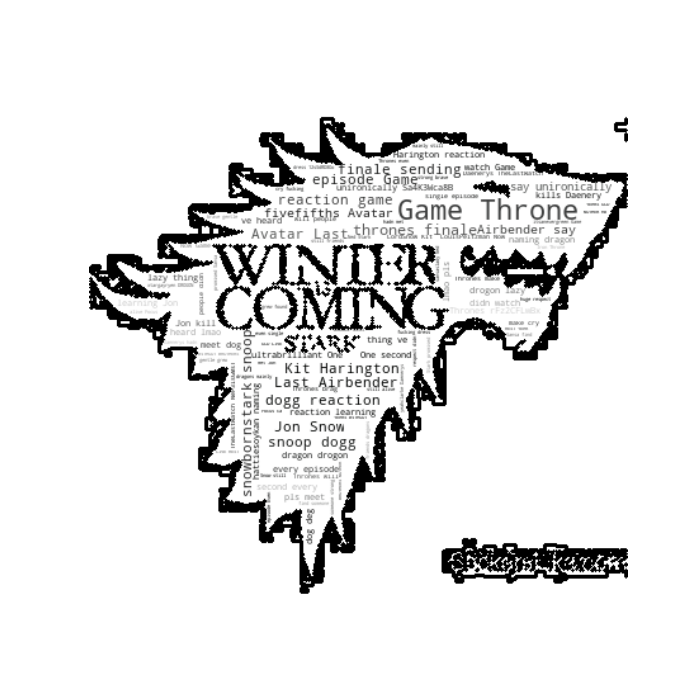
\includegraphics[scale=.7]{imagenes/JdTLogo.png}
	\caption{Wordcloud de Juego de Tronos}
	\label{fig:wordcloudJdT}
\end{figure} 


Cuya versión simplificada, más fácil de leer sería: 
\begin{figure}[H]
	\centering
	\includegraphics[scale=.9]{imagenes/JdTred.png}
	\caption{Wordcloud de Juego de Tronos simple}
	\label{fig:wordcloudJdT}
\end{figure} 

Una de las cosas que más llama la atención de este wordcloud fue la gran presencia de \"Avatar the Last Airbender\" y de \"Snoop Dogg\". Esto se debe a dos tweets diferentes publicados mientras se realizaba la captura de tweets, los cuales obtuvieron una enorme cantidad de Retweets y se almacenaron en la base de datos MongoDB miles de veces. 


\begin{figure}[H]
	\centering
	\begin{tabular}{c c}
		
		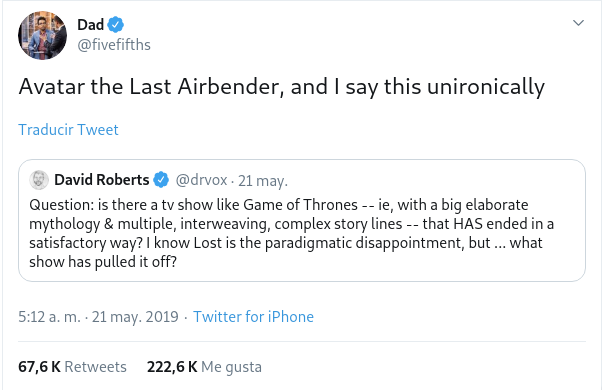
\includegraphics[scale=.3]{imagenes/airbender.png}
		&  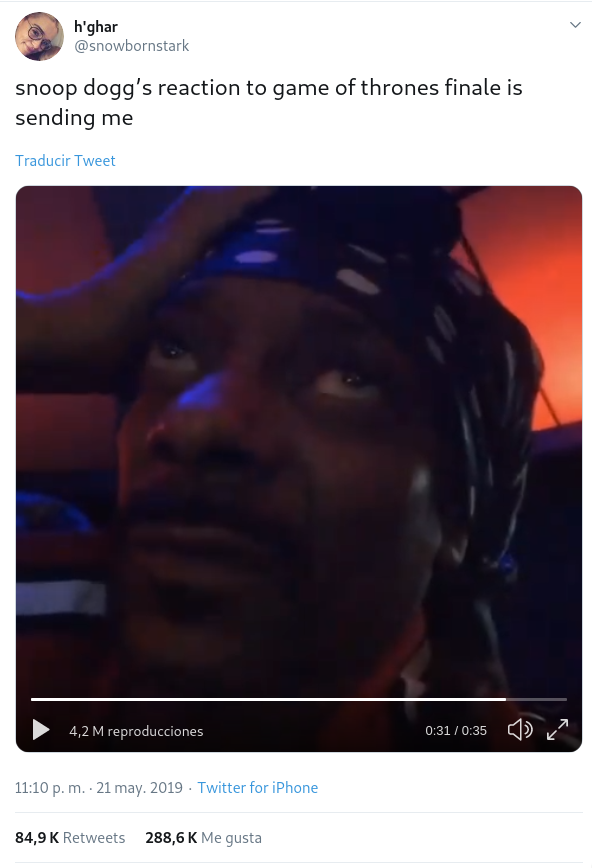
\includegraphics[scale=.3]{imagenes/snoop.png} \\ 
		
		{Tweet de Avatar Last Airbender}
		
		&  {Tweet sobre la reacción de Snoop Dogg} \\ 
		
	\end{tabular} 
	\caption{Tweets que tuvieron una alta tasa de Retweets y ensuciaron la base de datos}
	\label{fig:retweets}
\end{figure}


Y la forma que toman los 3500 tweets llevados a analizar a MeaningCloud es la siguiente:


\begin{table}[H]
	\centering
	\begin{tabular}{|c|c|c|}
		\hline 
		Polaridad& Suma de polaridades & Porcentaje \\ 
		\hline 
		N+& 286 & 26.19\% \\ 
		\hline 
		N& 253 &  29.61\%\\ 
		\hline 
		NEU& 19 & 1.97\% \\ 
		\hline 
		P& 379 & 39.234\% \\ 
		\hline 
		P+& 29 & 3.00\% \\ 
		\hline 
		Total & 6829 & \\
		\hline
	\end{tabular} 
	\caption{Tabla de porcentajes de análisis parcial de Juego de Tronos}
	\label{tbl:porcentaje-JdT}
\end{table}

\begin{figure}[H]
	\centering
	
		\includegraphics[scale=.3]{imagenes/barraJdt.png}
		
		\caption{Gráfico de barras de Juego de Tronos} 
		

	\label{fig:JdT}
\end{figure}

Lo más destacable es que los tweets muy negativos son muy altos, mucho más que en los demás datos obtenidos y la suma de ambos negativos supera con creces a la suma de las polaridades positivas, dejando clara que la tendencia en las redes es bastante negativa con respecto a Juego de Tronos. Lo cual se hizo patente fuera del proyecto, pues hubo un enorme descontento en las bases de los fans al final de la serie. Otro dato relevante es que los tweets sin tono emocional son muchos, esto se debe principalmente a que muchos de los tweets analizados estaban incompletos debido al modo de tweet extended. 
